\chapter{Model View Controler}

For our project as it were composed by a graphical user interface (UI), we have choose to implement a kind of model view controler pattern as seen in the figure \ref{mvc}.

  \begin{figure}[h!]
  \centering

  \scalebox{1}{
        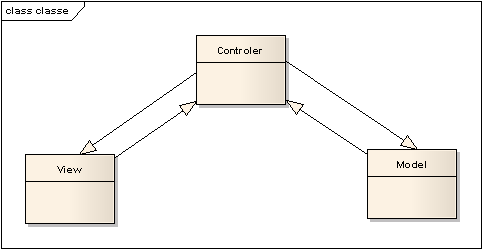
\includegraphics{image/MVCmodel}
  }

  \caption{Our MVC}
\label{mvc} 
 \end{figure}

As you will see on the diagram we not respect entirely the pattern. In the classical way of this pattern, the view is notified automatically if there is any change in the model, and the view directly ask the model of the change. In our way if the model change, the model tell the controler that tell the view, and the view ask the controler for the change.

All the transaction pass threw the controler, the controler is the kind of the master of the application it really make the links between the others perspective. 

All the action on the UI are transfert by actionListener to the controler that transfert to the model.

Our view is compose by the "fr.alma.ihm" package, this package containt all the graphical component for the UI.

Our controler is composed by the "fr.alma.controler" package, this package containt the controler, that "know" all the other perspective, and this package containt a factory, this factory is used to construct the different action listener.

Our model is composed by the "fr.alma.model" package, this package containt all the rule to play, the representation of the board and the class that is the AI.

Now we will see details about the different package and algorithm.


\clearpage
